\documentclass[1p]{elsarticle_modified}
%\bibliographystyle{elsarticle-num}

%\usepackage[colorlinks]{hyperref}
%\usepackage{abbrmath_seonhwa} %\Abb, \Ascr, \Acal ,\Abf, \Afrak
\usepackage{amsfonts}
\usepackage{amssymb}
\usepackage{amsmath}
\usepackage{amsthm}
\usepackage{scalefnt}
\usepackage{amsbsy}
\usepackage{kotex}
\usepackage{caption}
\usepackage{subfig}
\usepackage{color}
\usepackage{graphicx}
\usepackage{xcolor} %% white, black, red, green, blue, cyan, magenta, yellow
\usepackage{float}
\usepackage{setspace}
\usepackage{hyperref}

\usepackage{tikz}
\usetikzlibrary{arrows}

\usepackage{multirow}
\usepackage{array} % fixed length table
\usepackage{hhline}

%%%%%%%%%%%%%%%%%%%%%
\makeatletter
\renewcommand*\env@matrix[1][\arraystretch]{%
	\edef\arraystretch{#1}%
	\hskip -\arraycolsep
	\let\@ifnextchar\new@ifnextchar
	\array{*\c@MaxMatrixCols c}}
\makeatother %https://tex.stackexchange.com/questions/14071/how-can-i-increase-the-line-spacing-in-a-matrix
%%%%%%%%%%%%%%%

\usepackage[normalem]{ulem}

\newcommand{\msout}[1]{\ifmmode\text{\sout{\ensuremath{#1}}}\else\sout{#1}\fi}
%SOURCE: \msout is \stkout macro in https://tex.stackexchange.com/questions/20609/strikeout-in-math-mode

\newcommand{\cancel}[1]{
	\ifmmode
	{\color{red}\msout{#1}}
	\else
	{\color{red}\sout{#1}}
	\fi
}

\newcommand{\add}[1]{
	{\color{blue}\uwave{#1}}
}

\newcommand{\replace}[2]{
	\ifmmode
	{\color{red}\msout{#1}}{\color{blue}\uwave{#2}}
	\else
	{\color{red}\sout{#1}}{\color{blue}\uwave{#2}}
	\fi
}

\newcommand{\Sol}{\mathcal{S}} %segment
\newcommand{\D}{D} %diagram
\newcommand{\A}{\mathcal{A}} %arc


%%%%%%%%%%%%%%%%%%%%%%%%%%%%%5 test

\def\sl{\operatorname{\textup{SL}}(2,\Cbb)}
\def\psl{\operatorname{\textup{PSL}}(2,\Cbb)}
\def\quan{\mkern 1mu \triangleright \mkern 1mu}

\theoremstyle{definition}
\newtheorem{thm}{Theorem}[section]
\newtheorem{prop}[thm]{Proposition}
\newtheorem{lem}[thm]{Lemma}
\newtheorem{ques}[thm]{Question}
\newtheorem{cor}[thm]{Corollary}
\newtheorem{defn}[thm]{Definition}
\newtheorem{exam}[thm]{Example}
\newtheorem{rmk}[thm]{Remark}
\newtheorem{alg}[thm]{Algorithm}

\newcommand{\I}{\sqrt{-1}}
\begin{document}

%\begin{frontmatter}
%
%\title{Boundary parabolic representations of knots up to 8 crossings}
%
%%% Group authors per affiliation:
%\author{Yunhi Cho} 
%\address{Department of Mathematics, University of Seoul, Seoul, Korea}
%\ead{yhcho@uos.ac.kr}
%
%
%\author{Seonhwa Kim} %\fnref{s_kim}}
%\address{Center for Geometry and Physics, Institute for Basic Science, Pohang, 37673, Korea}
%\ead{ryeona17@ibs.re.kr}
%
%\author{Hyuk Kim}
%\address{Department of Mathematical Sciences, Seoul National University, Seoul 08826, Korea}
%\ead{hyukkim@snu.ac.kr}
%
%\author{Seokbeom Yoon}
%\address{Department of Mathematical Sciences, Seoul National University, Seoul, 08826,  Korea}
%\ead{sbyoon15@snu.ac.kr}
%
%\begin{abstract}
%We find all boundary parabolic representation of knots up to 8 crossings.
%
%\end{abstract}
%\begin{keyword}
%    \MSC[2010] 57M25 
%\end{keyword}
%
%\end{frontmatter}

%\linenumbers
%\tableofcontents
%
\newcommand\colored[1]{\textcolor{white}{\rule[-0.35ex]{0.8em}{1.4ex}}\kern-0.8em\color{red} #1}%
%\newcommand\colored[1]{\textcolor{white}{ #1}\kern-2.17ex	\textcolor{white}{ #1}\kern-1.81ex	\textcolor{white}{ #1}\kern-2.15ex\color{red}#1	}

{\Large $\underline{12n_{0513}~(K12n_{0513})}$}

\setlength{\tabcolsep}{10pt}
\renewcommand{\arraystretch}{1.6}
\vspace{1cm}\begin{tabular}{m{100pt}>{\centering\arraybackslash}m{274pt}}
\multirow{5}{120pt}{
	\centering
	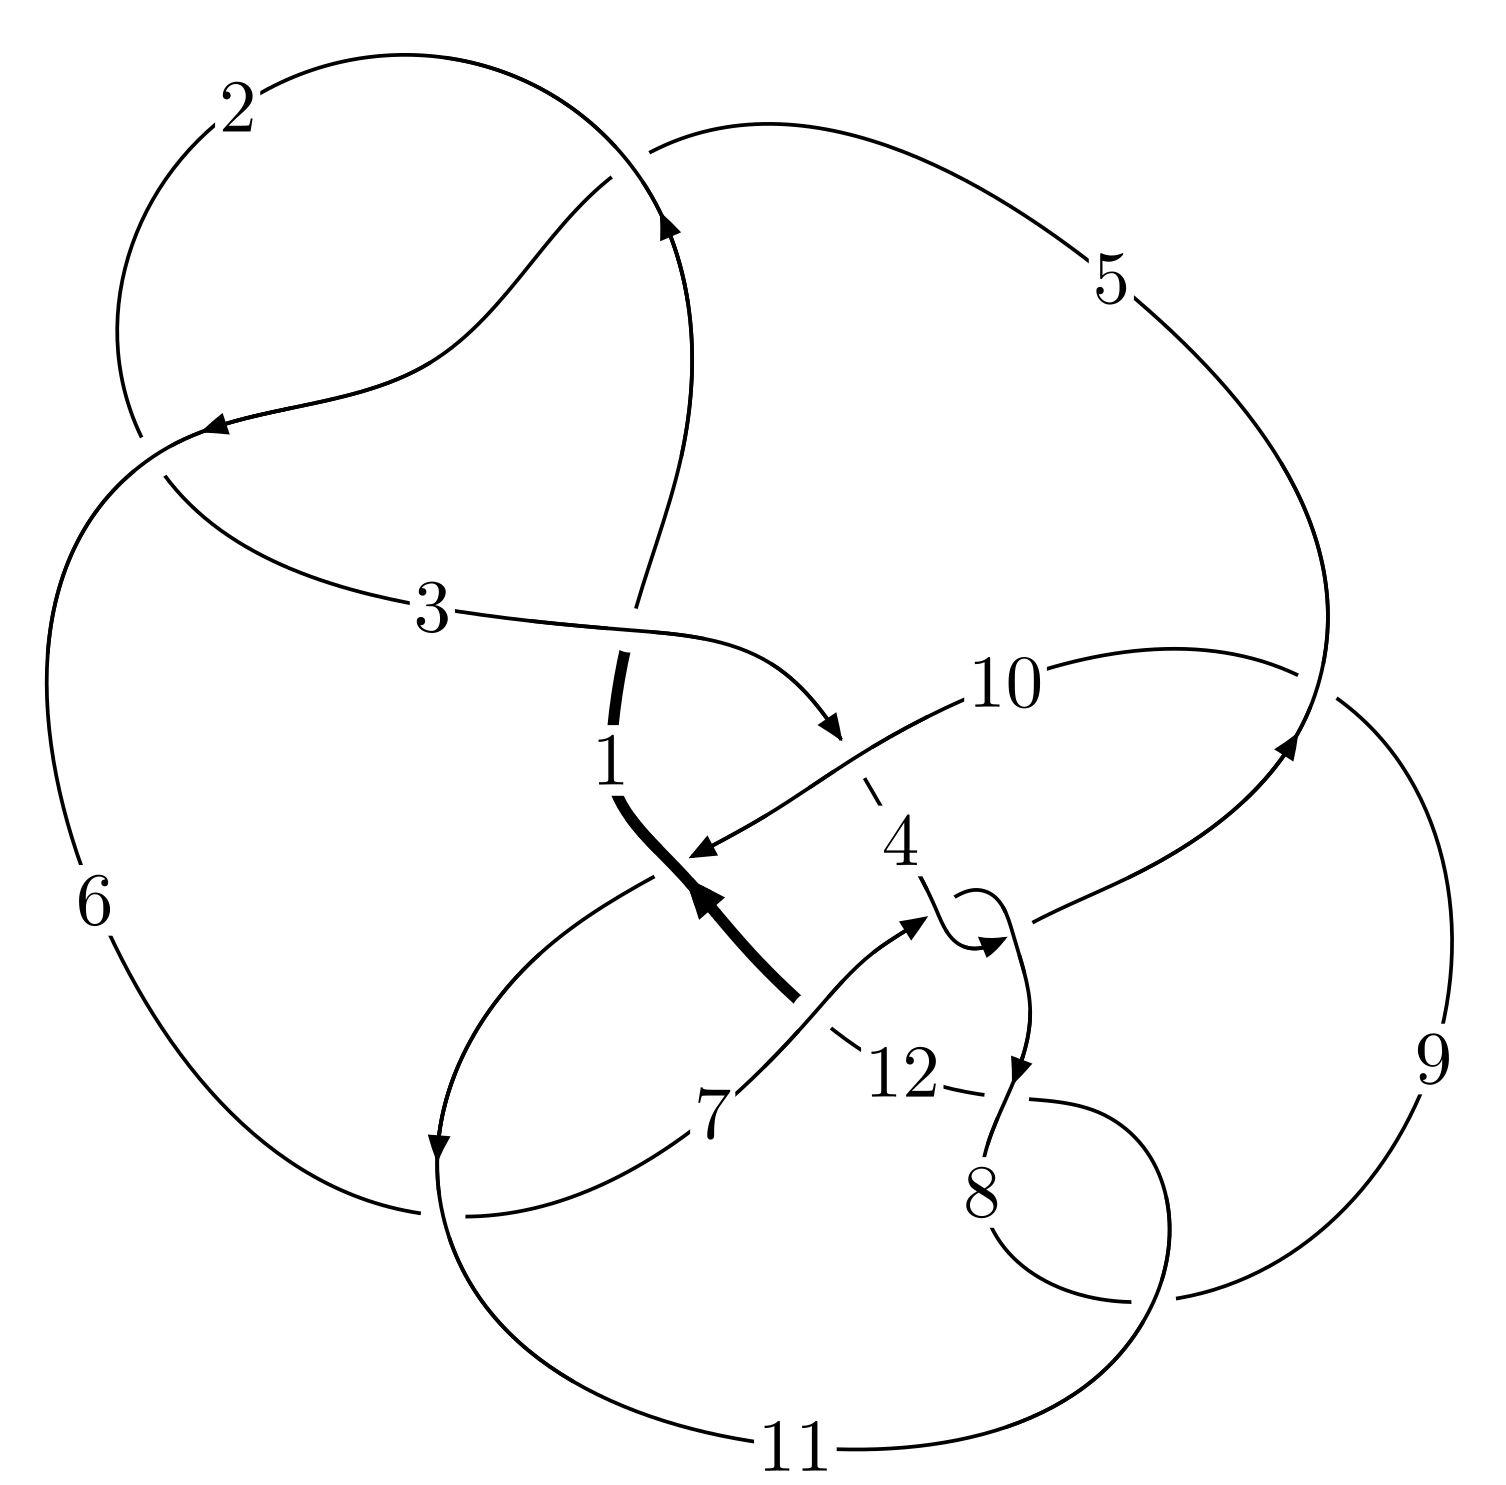
\includegraphics[width=112pt]{../../../GIT/diagram.site/Diagrams/png/2602_12n_0513.png}\\
\ \ \ A knot diagram\footnotemark}&
\allowdisplaybreaks
\textbf{Linearized knot diagam} \\
\cline{2-2}
 &
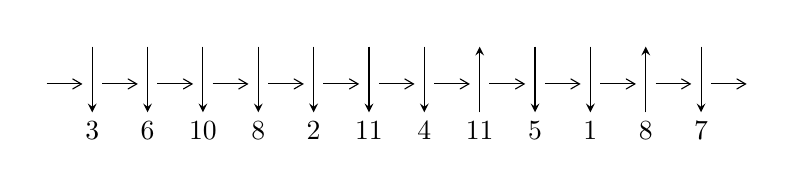
\begin{tikzpicture}[x=20pt, y=17pt]
	% nodes
	\node (C0) at (0, 0) {};
	\node (C1) at (1, 0) {};
	\node (C1U) at (1, +1) {};
	\node (C1D) at (1, -1) {3};

	\node (C2) at (2, 0) {};
	\node (C2U) at (2, +1) {};
	\node (C2D) at (2, -1) {6};

	\node (C3) at (3, 0) {};
	\node (C3U) at (3, +1) {};
	\node (C3D) at (3, -1) {10};

	\node (C4) at (4, 0) {};
	\node (C4U) at (4, +1) {};
	\node (C4D) at (4, -1) {8};

	\node (C5) at (5, 0) {};
	\node (C5U) at (5, +1) {};
	\node (C5D) at (5, -1) {2};

	\node (C6) at (6, 0) {};
	\node (C6U) at (6, +1) {};
	\node (C6D) at (6, -1) {11};

	\node (C7) at (7, 0) {};
	\node (C7U) at (7, +1) {};
	\node (C7D) at (7, -1) {4};

	\node (C8) at (8, 0) {};
	\node (C8U) at (8, +1) {};
	\node (C8D) at (8, -1) {11};

	\node (C9) at (9, 0) {};
	\node (C9U) at (9, +1) {};
	\node (C9D) at (9, -1) {5};

	\node (C10) at (10, 0) {};
	\node (C10U) at (10, +1) {};
	\node (C10D) at (10, -1) {1};

	\node (C11) at (11, 0) {};
	\node (C11U) at (11, +1) {};
	\node (C11D) at (11, -1) {8};

	\node (C12) at (12, 0) {};
	\node (C12U) at (12, +1) {};
	\node (C12D) at (12, -1) {7};
	\node (C13) at (13, 0) {};

	% arrows
	\draw[->,>={angle 60}]
	(C0) edge (C1) (C1) edge (C2) (C2) edge (C3) (C3) edge (C4) (C4) edge (C5) (C5) edge (C6) (C6) edge (C7) (C7) edge (C8) (C8) edge (C9) (C9) edge (C10) (C10) edge (C11) (C11) edge (C12) (C12) edge (C13) ;	\draw[->,>=stealth]
	(C1U) edge (C1D) (C2U) edge (C2D) (C3U) edge (C3D) (C4U) edge (C4D) (C5U) edge (C5D) (C6U) edge (C6D) (C7U) edge (C7D) (C8D) edge (C8U) (C9U) edge (C9D) (C10U) edge (C10D) (C11D) edge (C11U) (C12U) edge (C12D) ;
	\end{tikzpicture} \\
\hhline{~~} \\& 
\textbf{Solving Sequence} \\ \cline{2-2} 
 &
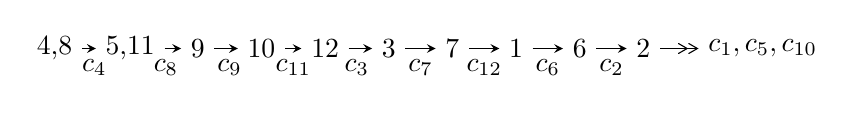
\begin{tikzpicture}[x=23pt, y=7pt]
	% node
	\node (A0) at (-1/8, 0) {4,8};
	\node (A1) at (17/16, 0) {5,11};
	\node (A2) at (17/8, 0) {9};
	\node (A3) at (25/8, 0) {10};
	\node (A4) at (33/8, 0) {12};
	\node (A5) at (41/8, 0) {3};
	\node (A6) at (49/8, 0) {7};
	\node (A7) at (57/8, 0) {1};
	\node (A8) at (65/8, 0) {6};
	\node (A9) at (73/8, 0) {2};
	\node (C1) at (1/2, -1) {$c_{4}$};
	\node (C2) at (13/8, -1) {$c_{8}$};
	\node (C3) at (21/8, -1) {$c_{9}$};
	\node (C4) at (29/8, -1) {$c_{11}$};
	\node (C5) at (37/8, -1) {$c_{3}$};
	\node (C6) at (45/8, -1) {$c_{7}$};
	\node (C7) at (53/8, -1) {$c_{12}$};
	\node (C8) at (61/8, -1) {$c_{6}$};
	\node (C9) at (69/8, -1) {$c_{2}$};
	\node (A10) at (11, 0) {$c_{1},c_{5},c_{10}$};

	% edge
	\draw[->,>=stealth]	
	(A0) edge (A1) (A1) edge (A2) (A2) edge (A3) (A3) edge (A4) (A4) edge (A5) (A5) edge (A6) (A6) edge (A7) (A7) edge (A8) (A8) edge (A9) ;
	\draw[->>,>={angle 60}]	
	(A9) edge (A10);
\end{tikzpicture} \\ 

\end{tabular} \\

\footnotetext{
The image of knot diagram is generated by the software ``\textbf{Draw programme}" developed by Andrew Bartholomew(\url{http://www.layer8.co.uk/maths/draw/index.htm\#Running-draw}), where we modified some parts for our purpose(\url{https://github.com/CATsTAILs/LinksPainter}).
}\phantom \\ \newline 
\centering \textbf{Ideals for irreducible components\footnotemark of $X_{\text{par}}$} 
 
\begin{align*}
I^u_{1}&=\langle 
-4.11455\times10^{216} u^{83}-1.22374\times10^{217} u^{82}+\cdots+1.43757\times10^{217} b-1.08508\times10^{217},\\
\phantom{I^u_{1}}&\phantom{= \langle  }-1.59930\times10^{217} u^{83}-4.98714\times10^{217} u^{82}+\cdots+1.43757\times10^{217} a-1.15733\times10^{218},\\
\phantom{I^u_{1}}&\phantom{= \langle  }u^{84}+3 u^{83}+\cdots+6 u-1\rangle \\
I^u_{2}&=\langle 
-2270 u^{21}-3510 u^{20}+\cdots+61 b-3235,\;-7325 u^{21}-11232 u^{20}+\cdots+61 a-11023,\\
\phantom{I^u_{2}}&\phantom{= \langle  }u^{22}+2 u^{21}+\cdots+3 u+1\rangle \\
\\
\end{align*}
\raggedright * 2 irreducible components of $\dim_{\mathbb{C}}=0$, with total 106 representations.\\
\footnotetext{All coefficients of polynomials are rational numbers. But the coefficients are sometimes approximated in decimal forms when there is not enough margin.}
\newpage
\renewcommand{\arraystretch}{1}
\centering \section*{I. $I^u_{1}= \langle -4.11\times10^{216} u^{83}-1.22\times10^{217} u^{82}+\cdots+1.44\times10^{217} b-1.09\times10^{217},\;-1.60\times10^{217} u^{83}-4.99\times10^{217} u^{82}+\cdots+1.44\times10^{217} a-1.16\times10^{218},\;u^{84}+3 u^{83}+\cdots+6 u-1 \rangle$}
\flushleft \textbf{(i) Arc colorings}\\
\begin{tabular}{m{7pt} m{180pt} m{7pt} m{180pt} }
\flushright $a_{4}=$&$\begin{pmatrix}1\\0\end{pmatrix}$ \\
\flushright $a_{8}=$&$\begin{pmatrix}0\\u\end{pmatrix}$ \\
\flushright $a_{5}=$&$\begin{pmatrix}1\\u^2\end{pmatrix}$ \\
\flushright $a_{11}=$&$\begin{pmatrix}1.11250 u^{83}+3.46914 u^{82}+\cdots-73.5902 u+8.05058\\0.286216 u^{83}+0.851258 u^{82}+\cdots-7.95580 u+0.754799\end{pmatrix}$ \\
\flushright $a_{9}=$&$\begin{pmatrix}2.00350 u^{83}+6.21549 u^{82}+\cdots-103.174 u+8.32630\\0.383700 u^{83}+1.12001 u^{82}+\cdots-7.13407 u+0.363188\end{pmatrix}$ \\
\flushright $a_{10}=$&$\begin{pmatrix}1.72740 u^{83}+5.47297 u^{82}+\cdots-95.2664 u+8.16810\\0.342545 u^{83}+1.03274 u^{82}+\cdots-7.92489 u+0.448974\end{pmatrix}$ \\
\flushright $a_{12}=$&$\begin{pmatrix}1.11250 u^{83}+3.46914 u^{82}+\cdots-73.5902 u+8.05058\\0.252151 u^{83}+0.812685 u^{82}+\cdots-8.27842 u+0.623153\end{pmatrix}$ \\
\flushright $a_{3}=$&$\begin{pmatrix}0.118293 u^{83}+0.140322 u^{82}+\cdots+28.7740 u+14.3613\\0.136975 u^{83}+0.450890 u^{82}+\cdots+0.649097 u+1.21041\end{pmatrix}$ \\
\flushright $a_{7}=$&$\begin{pmatrix}u\\u\end{pmatrix}$ \\
\flushright $a_{1}=$&$\begin{pmatrix}1.06394 u^{83}+3.26827 u^{82}+\cdots-73.1824 u+8.12599\\0.203595 u^{83}+0.611813 u^{82}+\cdots-7.87055 u+0.698566\end{pmatrix}$ \\
\flushright $a_{6}=$&$\begin{pmatrix}1.61980 u^{83}+5.09548 u^{82}+\cdots-94.0400 u+7.96311\\0.0171652 u^{83}+0.125743 u^{82}+\cdots-8.77587 u+0.619271\end{pmatrix}$ \\
\flushright $a_{2}=$&$\begin{pmatrix}-1.37298 u^{83}-4.14238 u^{82}+\cdots+83.9230 u+0.293934\\-0.122114 u^{83}-0.296643 u^{82}+\cdots+4.05853 u+0.483833\end{pmatrix}$\\&\end{tabular}
\flushleft \textbf{(ii) Obstruction class $= -1$}\\~\\
\flushleft \textbf{(iii) Cusp Shapes $= -1.46226 u^{83}-4.71452 u^{82}+\cdots+33.6541 u-9.62565$}\\~\\
\newpage\renewcommand{\arraystretch}{1}
\flushleft \textbf{(iv) u-Polynomials at the component}\newline \\
\begin{tabular}{m{50pt}|m{274pt}}
Crossings & \hspace{64pt}u-Polynomials at each crossing \\
\hline $$\begin{aligned}c_{1}\end{aligned}$$&$\begin{aligned}
&u^{84}+35 u^{83}+\cdots+55 u+1
\end{aligned}$\\
\hline $$\begin{aligned}c_{2},c_{5}\end{aligned}$$&$\begin{aligned}
&u^{84}+u^{83}+\cdots+9 u-1
\end{aligned}$\\
\hline $$\begin{aligned}c_{3}\end{aligned}$$&$\begin{aligned}
&u^{84}+2 u^{83}+\cdots-3150 u-863
\end{aligned}$\\
\hline $$\begin{aligned}c_{4},c_{7}\end{aligned}$$&$\begin{aligned}
&u^{84}+3 u^{83}+\cdots+6 u-1
\end{aligned}$\\
\hline $$\begin{aligned}c_{6}\end{aligned}$$&$\begin{aligned}
&u^{84}+u^{83}+\cdots-4996204 u-2395607
\end{aligned}$\\
\hline $$\begin{aligned}c_{8},c_{11}\end{aligned}$$&$\begin{aligned}
&u^{84}-10 u^{83}+\cdots+8180 u+3952
\end{aligned}$\\
\hline $$\begin{aligned}c_{9}\end{aligned}$$&$\begin{aligned}
&u^{84}+34 u^{82}+\cdots+1301846276 u+241946651
\end{aligned}$\\
\hline $$\begin{aligned}c_{10}\end{aligned}$$&$\begin{aligned}
&u^{84}-10 u^{83}+\cdots-248 u+1
\end{aligned}$\\
\hline $$\begin{aligned}c_{12}\end{aligned}$$&$\begin{aligned}
&u^{84}-4 u^{83}+\cdots-28586236 u+7588717
\end{aligned}$\\
\hline
\end{tabular}\\~\\
\newpage\renewcommand{\arraystretch}{1}
\flushleft \textbf{(v) Riley Polynomials at the component}\newline \\
\begin{tabular}{m{50pt}|m{274pt}}
Crossings & \hspace{64pt}Riley Polynomials at each crossing \\
\hline $$\begin{aligned}c_{1}\end{aligned}$$&$\begin{aligned}
&y^{84}+37 y^{83}+\cdots+1781 y+1
\end{aligned}$\\
\hline $$\begin{aligned}c_{2},c_{5}\end{aligned}$$&$\begin{aligned}
&y^{84}-35 y^{83}+\cdots-55 y+1
\end{aligned}$\\
\hline $$\begin{aligned}c_{3}\end{aligned}$$&$\begin{aligned}
&y^{84}+12 y^{83}+\cdots+9189498 y+744769
\end{aligned}$\\
\hline $$\begin{aligned}c_{4},c_{7}\end{aligned}$$&$\begin{aligned}
&y^{84}-21 y^{83}+\cdots+48 y+1
\end{aligned}$\\
\hline $$\begin{aligned}c_{6}\end{aligned}$$&$\begin{aligned}
&y^{84}+53 y^{83}+\cdots-69359144214586 y+5738932898449
\end{aligned}$\\
\hline $$\begin{aligned}c_{8},c_{11}\end{aligned}$$&$\begin{aligned}
&y^{84}-84 y^{83}+\cdots-1119037552 y+15618304
\end{aligned}$\\
\hline $$\begin{aligned}c_{9}\end{aligned}$$&$\begin{aligned}
&y^{84}+68 y^{83}+\cdots+1815122488070227036 y+58538181930115801
\end{aligned}$\\
\hline $$\begin{aligned}c_{10}\end{aligned}$$&$\begin{aligned}
&y^{84}+12 y^{83}+\cdots-58496 y+1
\end{aligned}$\\
\hline $$\begin{aligned}c_{12}\end{aligned}$$&$\begin{aligned}
&y^{84}+64 y^{83}+\cdots-298596197402654 y+57588625706089
\end{aligned}$\\
\hline
\end{tabular}\\~\\
\newpage\flushleft \textbf{(vi) Complex Volumes and Cusp Shapes}
$$\begin{array}{c|c|c}  
\text{Solutions to }I^u_{1}& \I (\text{vol} + \sqrt{-1}CS) & \text{Cusp shape}\\
 \hline 
\begin{aligned}
u &= \phantom{-}0.900153 + 0.297981 I \\
a &= \phantom{-}0.152850 - 0.484510 I \\
b &= \phantom{-}1.277690 - 0.223754 I\end{aligned}
 & -0.21302 - 4.33780 I & \phantom{-0.000000 } 0 \\ \hline\begin{aligned}
u &= \phantom{-}0.900153 - 0.297981 I \\
a &= \phantom{-}0.152850 + 0.484510 I \\
b &= \phantom{-}1.277690 + 0.223754 I\end{aligned}
 & -0.21302 + 4.33780 I & \phantom{-0.000000 } 0 \\ \hline\begin{aligned}
u &= -0.721646 + 0.828109 I \\
a &= -0.479477 - 1.213880 I \\
b &= -0.562940 - 0.435217 I\end{aligned}
 & \phantom{-}2.62706 + 3.30026 I & \phantom{-0.000000 } 0 \\ \hline\begin{aligned}
u &= -0.721646 - 0.828109 I \\
a &= -0.479477 + 1.213880 I \\
b &= -0.562940 + 0.435217 I\end{aligned}
 & \phantom{-}2.62706 - 3.30026 I & \phantom{-0.000000 } 0 \\ \hline\begin{aligned}
u &= \phantom{-}0.898980 + 0.044549 I \\
a &= \phantom{-}0.520925 - 1.086290 I \\
b &= \phantom{-}1.39226 - 1.50003 I\end{aligned}
 & -0.92412 - 1.22946 I & -12.54684 + 0. I\phantom{ +0.000000I} \\ \hline\begin{aligned}
u &= \phantom{-}0.898980 - 0.044549 I \\
a &= \phantom{-}0.520925 + 1.086290 I \\
b &= \phantom{-}1.39226 + 1.50003 I\end{aligned}
 & -0.92412 + 1.22946 I & -12.54684 + 0. I\phantom{ +0.000000I} \\ \hline\begin{aligned}
u &= -0.881658 + 0.085784 I \\
a &= -0.628035 + 1.224740 I \\
b &= -1.12816 + 2.00117 I\end{aligned}
 & -1.65718 - 5.58665 I & -13.05862 + 4.36644 I \\ \hline\begin{aligned}
u &= -0.881658 - 0.085784 I \\
a &= -0.628035 - 1.224740 I \\
b &= -1.12816 - 2.00117 I\end{aligned}
 & -1.65718 + 5.58665 I & -13.05862 - 4.36644 I \\ \hline\begin{aligned}
u &= -0.780154 + 0.371808 I \\
a &= \phantom{-}0.156738 - 0.240422 I \\
b &= -0.771810 + 0.080467 I\end{aligned}
 & -0.0845697 - 0.1001390 I & -9.69562 + 0. I\phantom{ +0.000000I} \\ \hline\begin{aligned}
u &= -0.780154 - 0.371808 I \\
a &= \phantom{-}0.156738 + 0.240422 I \\
b &= -0.771810 - 0.080467 I\end{aligned}
 & -0.0845697 + 0.1001390 I & -9.69562 + 0. I\phantom{ +0.000000I}\\
 \hline 
 \end{array}$$\newpage$$\begin{array}{c|c|c}  
\text{Solutions to }I^u_{1}& \I (\text{vol} + \sqrt{-1}CS) & \text{Cusp shape}\\
 \hline 
\begin{aligned}
u &= -0.826574 + 0.108876 I \\
a &= \phantom{-}0.648654 + 0.935247 I \\
b &= -0.312333 + 0.007656 I\end{aligned}
 & \phantom{-}0.214695 - 0.733341 I & -9.75722 - 1.67126 I \\ \hline\begin{aligned}
u &= -0.826574 - 0.108876 I \\
a &= \phantom{-}0.648654 - 0.935247 I \\
b &= -0.312333 - 0.007656 I\end{aligned}
 & \phantom{-}0.214695 + 0.733341 I & -9.75722 + 1.67126 I \\ \hline\begin{aligned}
u &= -0.870921 + 0.787220 I \\
a &= -0.60547 - 1.61811 I \\
b &= -1.43008 - 1.28544 I\end{aligned}
 & \phantom{-}5.63391 + 7.36950 I & \phantom{-0.000000 } 0 \\ \hline\begin{aligned}
u &= -0.870921 - 0.787220 I \\
a &= -0.60547 + 1.61811 I \\
b &= -1.43008 + 1.28544 I\end{aligned}
 & \phantom{-}5.63391 - 7.36950 I & \phantom{-0.000000 } 0 \\ \hline\begin{aligned}
u &= -0.917337 + 0.733359 I \\
a &= -1.35773 - 0.70979 I \\
b &= -1.61122 - 0.13239 I\end{aligned}
 & \phantom{-}5.47056 - 1.58629 I & \phantom{-0.000000 } 0 \\ \hline\begin{aligned}
u &= -0.917337 - 0.733359 I \\
a &= -1.35773 + 0.70979 I \\
b &= -1.61122 + 0.13239 I\end{aligned}
 & \phantom{-}5.47056 + 1.58629 I & \phantom{-0.000000 } 0 \\ \hline\begin{aligned}
u &= -0.698347 + 0.435308 I \\
a &= \phantom{-}1.19604 - 1.25661 I \\
b &= -0.330618 - 1.054550 I\end{aligned}
 & -3.52883 + 2.77312 I & -15.4506 - 6.7979 I \\ \hline\begin{aligned}
u &= -0.698347 - 0.435308 I \\
a &= \phantom{-}1.19604 + 1.25661 I \\
b &= -0.330618 + 1.054550 I\end{aligned}
 & -3.52883 - 2.77312 I & -15.4506 + 6.7979 I \\ \hline\begin{aligned}
u &= -0.071228 + 0.808709 I \\
a &= \phantom{-}0.684407 - 0.392922 I \\
b &= -0.667491 + 0.370099 I\end{aligned}
 & \phantom{-}2.08277 + 3.57421 I & -4.77531 - 3.69472 I \\ \hline\begin{aligned}
u &= -0.071228 - 0.808709 I \\
a &= \phantom{-}0.684407 + 0.392922 I \\
b &= -0.667491 - 0.370099 I\end{aligned}
 & \phantom{-}2.08277 - 3.57421 I & -4.77531 + 3.69472 I\\
 \hline 
 \end{array}$$\newpage$$\begin{array}{c|c|c}  
\text{Solutions to }I^u_{1}& \I (\text{vol} + \sqrt{-1}CS) & \text{Cusp shape}\\
 \hline 
\begin{aligned}
u &= \phantom{-}0.882596 + 0.809217 I \\
a &= \phantom{-}0.76923 - 1.57559 I \\
b &= \phantom{-}1.68260 - 1.03445 I\end{aligned}
 & \phantom{-}6.12462 - 2.40868 I & \phantom{-0.000000 } 0 \\ \hline\begin{aligned}
u &= \phantom{-}0.882596 - 0.809217 I \\
a &= \phantom{-}0.76923 + 1.57559 I \\
b &= \phantom{-}1.68260 + 1.03445 I\end{aligned}
 & \phantom{-}6.12462 + 2.40868 I & \phantom{-0.000000 } 0 \\ \hline\begin{aligned}
u &= \phantom{-}0.919192 + 0.775802 I \\
a &= \phantom{-}1.27737 - 0.97215 I \\
b &= \phantom{-}1.77985 - 0.24242 I\end{aligned}
 & \phantom{-}6.00052 - 3.56886 I & \phantom{-0.000000 } 0 \\ \hline\begin{aligned}
u &= \phantom{-}0.919192 - 0.775802 I \\
a &= \phantom{-}1.27737 + 0.97215 I \\
b &= \phantom{-}1.77985 + 0.24242 I\end{aligned}
 & \phantom{-}6.00052 + 3.56886 I & \phantom{-0.000000 } 0 \\ \hline\begin{aligned}
u &= -0.131087 + 0.779739 I \\
a &= -0.618512 - 0.563874 I \\
b &= \phantom{-}0.623447 + 0.478283 I\end{aligned}
 & \phantom{-}2.93571 + 1.52852 I & -2.60851 - 2.55303 I \\ \hline\begin{aligned}
u &= -0.131087 - 0.779739 I \\
a &= -0.618512 + 0.563874 I \\
b &= \phantom{-}0.623447 - 0.478283 I\end{aligned}
 & \phantom{-}2.93571 - 1.52852 I & -2.60851 + 2.55303 I \\ \hline\begin{aligned}
u &= -0.532846 + 0.536929 I \\
a &= -0.110446 - 0.772642 I \\
b &= \phantom{-}1.039160 - 0.278861 I\end{aligned}
 & \phantom{-}1.53936 + 3.45140 I & -4.45971 - 6.29986 I \\ \hline\begin{aligned}
u &= -0.532846 - 0.536929 I \\
a &= -0.110446 + 0.772642 I \\
b &= \phantom{-}1.039160 + 0.278861 I\end{aligned}
 & \phantom{-}1.53936 - 3.45140 I & -4.45971 + 6.29986 I \\ \hline\begin{aligned}
u &= \phantom{-}0.743015 + 0.118915 I \\
a &= -1.08667 + 1.31261 I \\
b &= \phantom{-}0.311075 + 0.036329 I\end{aligned}
 & -1.00616 + 6.17268 I & -13.15706 - 1.64571 I \\ \hline\begin{aligned}
u &= \phantom{-}0.743015 - 0.118915 I \\
a &= -1.08667 - 1.31261 I \\
b &= \phantom{-}0.311075 - 0.036329 I\end{aligned}
 & -1.00616 - 6.17268 I & -13.15706 + 1.64571 I\\
 \hline 
 \end{array}$$\newpage$$\begin{array}{c|c|c}  
\text{Solutions to }I^u_{1}& \I (\text{vol} + \sqrt{-1}CS) & \text{Cusp shape}\\
 \hline 
\begin{aligned}
u &= \phantom{-}0.608571 + 0.441527 I \\
a &= -0.116760 - 0.757237 I \\
b &= -1.50360 - 0.59788 I\end{aligned}
 & -0.30762 - 8.50634 I & -8.7735 + 11.8688 I \\ \hline\begin{aligned}
u &= \phantom{-}0.608571 - 0.441527 I \\
a &= -0.116760 + 0.757237 I \\
b &= -1.50360 + 0.59788 I\end{aligned}
 & -0.30762 + 8.50634 I & -8.7735 - 11.8688 I \\ \hline\begin{aligned}
u &= -0.763077 + 1.009160 I \\
a &= \phantom{-}0.290491 + 1.008800 I \\
b &= \phantom{-}1.26873 + 0.94425 I\end{aligned}
 & \phantom{-}5.88830 + 7.20760 I & \phantom{-0.000000 } 0 \\ \hline\begin{aligned}
u &= -0.763077 - 1.009160 I \\
a &= \phantom{-}0.290491 - 1.008800 I \\
b &= \phantom{-}1.26873 - 0.94425 I\end{aligned}
 & \phantom{-}5.88830 - 7.20760 I & \phantom{-0.000000 } 0 \\ \hline\begin{aligned}
u &= \phantom{-}0.718688\phantom{ +0.000000I} \\
a &= -1.57675\phantom{ +0.000000I} \\
b &= \phantom{-}0.296620\phantom{ +0.000000I}\end{aligned}
 & -5.24836\phantom{ +0.000000I} & -19.9760\phantom{ +0.000000I} \\ \hline\begin{aligned}
u &= \phantom{-}0.935696 + 0.904486 I \\
a &= \phantom{-}0.732618 - 1.149590 I \\
b &= \phantom{-}1.70260 - 0.35455 I\end{aligned}
 & \phantom{-}4.37832 - 3.33219 I & \phantom{-0.000000 } 0 \\ \hline\begin{aligned}
u &= \phantom{-}0.935696 - 0.904486 I \\
a &= \phantom{-}0.732618 + 1.149590 I \\
b &= \phantom{-}1.70260 + 0.35455 I\end{aligned}
 & \phantom{-}4.37832 + 3.33219 I & \phantom{-0.000000 } 0 \\ \hline\begin{aligned}
u &= \phantom{-}0.795821 + 1.049650 I \\
a &= -0.428636 + 0.975134 I \\
b &= -1.31864 + 0.60090 I\end{aligned}
 & \phantom{-}8.06712 - 0.99861 I & \phantom{-0.000000 } 0 \\ \hline\begin{aligned}
u &= \phantom{-}0.795821 - 1.049650 I \\
a &= -0.428636 - 0.975134 I \\
b &= -1.31864 - 0.60090 I\end{aligned}
 & \phantom{-}8.06712 + 0.99861 I & \phantom{-0.000000 } 0 \\ \hline\begin{aligned}
u &= -0.483252 + 0.480273 I \\
a &= \phantom{-}1.88640 - 2.27246 I \\
b &= -0.558902 - 1.166930 I\end{aligned}
 & \phantom{-}0.09901 + 7.96107 I & -7.32121 - 11.83227 I\\
 \hline 
 \end{array}$$\newpage$$\begin{array}{c|c|c}  
\text{Solutions to }I^u_{1}& \I (\text{vol} + \sqrt{-1}CS) & \text{Cusp shape}\\
 \hline 
\begin{aligned}
u &= -0.483252 - 0.480273 I \\
a &= \phantom{-}1.88640 + 2.27246 I \\
b &= -0.558902 + 1.166930 I\end{aligned}
 & \phantom{-}0.09901 - 7.96107 I & -7.32121 + 11.83227 I \\ \hline\begin{aligned}
u &= -0.616946 + 0.250802 I \\
a &= -0.74826 + 1.21205 I \\
b &= -0.19427 + 1.83238 I\end{aligned}
 & -3.45151 + 0.05717 I & -15.3703 - 3.3052 I \\ \hline\begin{aligned}
u &= -0.616946 - 0.250802 I \\
a &= -0.74826 - 1.21205 I \\
b &= -0.19427 - 1.83238 I\end{aligned}
 & -3.45151 - 0.05717 I & -15.3703 + 3.3052 I \\ \hline\begin{aligned}
u &= -0.799101 + 1.075390 I \\
a &= \phantom{-}0.589749 + 0.783838 I \\
b &= \phantom{-}0.951424 + 0.130937 I\end{aligned}
 & \phantom{-}1.72718 - 2.24494 I & \phantom{-0.000000 } 0 \\ \hline\begin{aligned}
u &= -0.799101 - 1.075390 I \\
a &= \phantom{-}0.589749 - 0.783838 I \\
b &= \phantom{-}0.951424 - 0.130937 I\end{aligned}
 & \phantom{-}1.72718 + 2.24494 I & \phantom{-0.000000 } 0 \\ \hline\begin{aligned}
u &= -0.709874 + 1.145940 I \\
a &= -0.707557 - 1.188160 I \\
b &= -1.16025 + 0.97520 I\end{aligned}
 & \phantom{-}5.83263 - 0.09887 I & \phantom{-0.000000 } 0 \\ \hline\begin{aligned}
u &= -0.709874 - 1.145940 I \\
a &= -0.707557 + 1.188160 I \\
b &= -1.16025 - 0.97520 I\end{aligned}
 & \phantom{-}5.83263 + 0.09887 I & \phantom{-0.000000 } 0 \\ \hline\begin{aligned}
u &= -1.113350 + 0.768279 I \\
a &= -0.620139 - 0.681105 I \\
b &= -1.55359 - 0.74336 I\end{aligned}
 & \phantom{-}1.39386 + 2.74337 I & \phantom{-0.000000 } 0 \\ \hline\begin{aligned}
u &= -1.113350 - 0.768279 I \\
a &= -0.620139 + 0.681105 I \\
b &= -1.55359 + 0.74336 I\end{aligned}
 & \phantom{-}1.39386 - 2.74337 I & \phantom{-0.000000 } 0 \\ \hline\begin{aligned}
u &= -1.344250 + 0.217412 I \\
a &= \phantom{-}0.191483 + 0.020332 I \\
b &= \phantom{-}0.162753 - 0.595444 I\end{aligned}
 & -1.31503 + 2.43238 I & \phantom{-0.000000 } 0\\
 \hline 
 \end{array}$$\newpage$$\begin{array}{c|c|c}  
\text{Solutions to }I^u_{1}& \I (\text{vol} + \sqrt{-1}CS) & \text{Cusp shape}\\
 \hline 
\begin{aligned}
u &= -1.344250 - 0.217412 I \\
a &= \phantom{-}0.191483 - 0.020332 I \\
b &= \phantom{-}0.162753 + 0.595444 I\end{aligned}
 & -1.31503 - 2.43238 I & \phantom{-0.000000 } 0 \\ \hline\begin{aligned}
u &= \phantom{-}0.816860 + 1.100600 I \\
a &= -0.723679 + 0.953539 I \\
b &= -1.42267 - 0.16761 I\end{aligned}
 & \phantom{-}8.92473 + 4.08371 I & \phantom{-0.000000 } 0 \\ \hline\begin{aligned}
u &= \phantom{-}0.816860 - 1.100600 I \\
a &= -0.723679 - 0.953539 I \\
b &= -1.42267 + 0.16761 I\end{aligned}
 & \phantom{-}8.92473 - 4.08371 I & \phantom{-0.000000 } 0 \\ \hline\begin{aligned}
u &= -0.810679 + 1.116350 I \\
a &= \phantom{-}0.795718 + 0.932947 I \\
b &= \phantom{-}1.38186 - 0.37607 I\end{aligned}
 & \phantom{-}7.28558 - 10.07310 I & \phantom{-0.000000 } 0 \\ \hline\begin{aligned}
u &= -0.810679 - 1.116350 I \\
a &= \phantom{-}0.795718 - 0.932947 I \\
b &= \phantom{-}1.38186 + 0.37607 I\end{aligned}
 & \phantom{-}7.28558 + 10.07310 I & \phantom{-0.000000 } 0 \\ \hline\begin{aligned}
u &= \phantom{-}0.452766 + 0.404638 I \\
a &= -1.47433 - 2.68024 I \\
b &= \phantom{-}0.535538 - 1.093260 I\end{aligned}
 & \phantom{-}1.00688 - 2.77629 I & -4.92596 + 6.43001 I \\ \hline\begin{aligned}
u &= \phantom{-}0.452766 - 0.404638 I \\
a &= -1.47433 + 2.68024 I \\
b &= \phantom{-}0.535538 + 1.093260 I\end{aligned}
 & \phantom{-}1.00688 + 2.77629 I & -4.92596 - 6.43001 I \\ \hline\begin{aligned}
u &= \phantom{-}0.805308 + 1.153490 I \\
a &= \phantom{-}0.670849 - 1.225990 I \\
b &= \phantom{-}1.62167 + 0.83385 I\end{aligned}
 & \phantom{-}6.06561 - 4.85072 I & \phantom{-0.000000 } 0 \\ \hline\begin{aligned}
u &= \phantom{-}0.805308 - 1.153490 I \\
a &= \phantom{-}0.670849 + 1.225990 I \\
b &= \phantom{-}1.62167 - 0.83385 I\end{aligned}
 & \phantom{-}6.06561 + 4.85072 I & \phantom{-0.000000 } 0 \\ \hline\begin{aligned}
u &= \phantom{-}0.572850 + 0.113813 I \\
a &= \phantom{-}0.31165 - 1.93224 I \\
b &= \phantom{-}0.522800 - 1.239640 I\end{aligned}
 & -0.74994 - 2.26614 I & -2.36898 + 2.26109 I\\
 \hline 
 \end{array}$$\newpage$$\begin{array}{c|c|c}  
\text{Solutions to }I^u_{1}& \I (\text{vol} + \sqrt{-1}CS) & \text{Cusp shape}\\
 \hline 
\begin{aligned}
u &= \phantom{-}0.572850 - 0.113813 I \\
a &= \phantom{-}0.31165 + 1.93224 I \\
b &= \phantom{-}0.522800 + 1.239640 I\end{aligned}
 & -0.74994 + 2.26614 I & -2.36898 - 2.26109 I \\ \hline\begin{aligned}
u &= -1.10949 + 0.90861 I \\
a &= \phantom{-}0.575846 + 0.933832 I \\
b &= \phantom{-}1.43129 + 0.81182 I\end{aligned}
 & \phantom{-}0.73551 + 9.43744 I & \phantom{-0.000000 } 0 \\ \hline\begin{aligned}
u &= -1.10949 - 0.90861 I \\
a &= \phantom{-}0.575846 - 0.933832 I \\
b &= \phantom{-}1.43129 - 0.81182 I\end{aligned}
 & \phantom{-}0.73551 - 9.43744 I & \phantom{-0.000000 } 0 \\ \hline\begin{aligned}
u &= \phantom{-}1.12332 + 0.90477 I \\
a &= -0.794206 + 0.775788 I \\
b &= -1.384030 + 0.239354 I\end{aligned}
 & \phantom{-}7.03396 - 6.13444 I & \phantom{-0.000000 } 0 \\ \hline\begin{aligned}
u &= \phantom{-}1.12332 - 0.90477 I \\
a &= -0.794206 - 0.775788 I \\
b &= -1.384030 - 0.239354 I\end{aligned}
 & \phantom{-}7.03396 + 6.13444 I & \phantom{-0.000000 } 0 \\ \hline\begin{aligned}
u &= \phantom{-}1.11834 + 0.91483 I \\
a &= -0.698998 + 1.111010 I \\
b &= -1.93787 + 0.75793 I\end{aligned}
 & \phantom{-}7.93180 - 11.37730 I & \phantom{-0.000000 } 0 \\ \hline\begin{aligned}
u &= \phantom{-}1.11834 - 0.91483 I \\
a &= -0.698998 - 1.111010 I \\
b &= -1.93787 - 0.75793 I\end{aligned}
 & \phantom{-}7.93180 + 11.37730 I & \phantom{-0.000000 } 0 \\ \hline\begin{aligned}
u &= \phantom{-}1.44736\phantom{ +0.000000I} \\
a &= -0.363781\phantom{ +0.000000I} \\
b &= -0.569357\phantom{ +0.000000I}\end{aligned}
 & -7.28072\phantom{ +0.000000I} & \phantom{-0.000000 } 0 \\ \hline\begin{aligned}
u &= -1.12433 + 0.91467 I \\
a &= \phantom{-}0.648636 + 1.173700 I \\
b &= \phantom{-}2.02318 + 0.93554 I\end{aligned}
 & \phantom{-}6.2467 + 17.4034 I & \phantom{-0.000000 } 0 \\ \hline\begin{aligned}
u &= -1.12433 - 0.91467 I \\
a &= \phantom{-}0.648636 - 1.173700 I \\
b &= \phantom{-}2.02318 - 0.93554 I\end{aligned}
 & \phantom{-}6.2467 - 17.4034 I & \phantom{-0.000000 } 0\\
 \hline 
 \end{array}$$\newpage$$\begin{array}{c|c|c}  
\text{Solutions to }I^u_{1}& \I (\text{vol} + \sqrt{-1}CS) & \text{Cusp shape}\\
 \hline 
\begin{aligned}
u &= -1.16723 + 0.87243 I \\
a &= \phantom{-}0.832601 + 0.550806 I \\
b &= \phantom{-}1.073570 - 0.015326 I\end{aligned}
 & \phantom{-}4.64251 - 0.27243 I & \phantom{-0.000000 } 0 \\ \hline\begin{aligned}
u &= -1.16723 - 0.87243 I \\
a &= \phantom{-}0.832601 - 0.550806 I \\
b &= \phantom{-}1.073570 + 0.015326 I\end{aligned}
 & \phantom{-}4.64251 + 0.27243 I & \phantom{-0.000000 } 0 \\ \hline\begin{aligned}
u &= \phantom{-}1.46004 + 0.25246 I \\
a &= -0.241739 - 0.095073 I \\
b &= -0.433386 - 0.864185 I\end{aligned}
 & -3.27457 - 7.84836 I & \phantom{-0.000000 } 0 \\ \hline\begin{aligned}
u &= \phantom{-}1.46004 - 0.25246 I \\
a &= -0.241739 + 0.095073 I \\
b &= -0.433386 + 0.864185 I\end{aligned}
 & -3.27457 + 7.84836 I & \phantom{-0.000000 } 0 \\ \hline\begin{aligned}
u &= \phantom{-}0.360098 + 0.364687 I \\
a &= \phantom{-}0.126184 - 0.361675 I \\
b &= -1.58298 + 0.61850 I\end{aligned}
 & -3.32779 - 1.11831 I & -1.97095 + 8.18187 I \\ \hline\begin{aligned}
u &= \phantom{-}0.360098 - 0.364687 I \\
a &= \phantom{-}0.126184 + 0.361675 I \\
b &= -1.58298 - 0.61850 I\end{aligned}
 & -3.32779 + 1.11831 I & -1.97095 - 8.18187 I \\ \hline\begin{aligned}
u &= \phantom{-}1.09967 + 1.02790 I \\
a &= \phantom{-}0.499291 - 1.100540 I \\
b &= \phantom{-}2.35471 - 0.43931 I\end{aligned}
 & \phantom{-}5.16143 - 2.94606 I & \phantom{-0.000000 } 0 \\ \hline\begin{aligned}
u &= \phantom{-}1.09967 - 1.02790 I \\
a &= \phantom{-}0.499291 + 1.100540 I \\
b &= \phantom{-}2.35471 + 0.43931 I\end{aligned}
 & \phantom{-}5.16143 + 2.94606 I & \phantom{-0.000000 } 0 \\ \hline\begin{aligned}
u &= -0.483190\phantom{ +0.000000I} \\
a &= \phantom{-}0.389799\phantom{ +0.000000I} \\
b &= -0.350552\phantom{ +0.000000I}\end{aligned}
 & -0.728767\phantom{ +0.000000I} & -13.5780\phantom{ +0.000000I} \\ \hline\begin{aligned}
u &= \phantom{-}1.54161\phantom{ +0.000000I} \\
a &= -0.494347\phantom{ +0.000000I} \\
b &= -0.315152\phantom{ +0.000000I}\end{aligned}
 & -7.66030\phantom{ +0.000000I} & \phantom{-0.000000 } 0\\
 \hline 
 \end{array}$$\newpage$$\begin{array}{c|c|c}  
\text{Solutions to }I^u_{1}& \I (\text{vol} + \sqrt{-1}CS) & \text{Cusp shape}\\
 \hline 
\begin{aligned}
u &= -1.18837 + 0.98534 I \\
a &= -0.407590 - 1.019860 I \\
b &= -2.35923 - 0.86528 I\end{aligned}
 & \phantom{-}4.38461 + 7.76770 I & \phantom{-0.000000 } 0 \\ \hline\begin{aligned}
u &= -1.18837 - 0.98534 I \\
a &= -0.407590 + 1.019860 I \\
b &= -2.35923 + 0.86528 I\end{aligned}
 & \phantom{-}4.38461 - 7.76770 I & \phantom{-0.000000 } 0 \\ \hline\begin{aligned}
u &= \phantom{-}0.0562391 + 0.1093170 I \\
a &= \phantom{-}3.31304 - 10.80210 I \\
b &= \phantom{-}0.057086 - 0.925377 I\end{aligned}
 & \phantom{-}2.98085 - 2.73185 I & -6.71068 + 3.58075 I \\ \hline\begin{aligned}
u &= \phantom{-}0.0562391 - 0.1093170 I \\
a &= \phantom{-}3.31304 + 10.80210 I \\
b &= \phantom{-}0.057086 + 0.925377 I\end{aligned}
 & \phantom{-}2.98085 + 2.73185 I & -6.71068 - 3.58075 I\\
 \hline 
 \end{array}$$\newpage\newpage\renewcommand{\arraystretch}{1}
\centering \section*{II. $I^u_{2}= \langle -2270 u^{21}-3510 u^{20}+\cdots+61 b-3235,\;-7325 u^{21}-11232 u^{20}+\cdots+61 a-11023,\;u^{22}+2 u^{21}+\cdots+3 u+1 \rangle$}
\flushleft \textbf{(i) Arc colorings}\\
\begin{tabular}{m{7pt} m{180pt} m{7pt} m{180pt} }
\flushright $a_{4}=$&$\begin{pmatrix}1\\0\end{pmatrix}$ \\
\flushright $a_{8}=$&$\begin{pmatrix}0\\u\end{pmatrix}$ \\
\flushright $a_{5}=$&$\begin{pmatrix}1\\u^2\end{pmatrix}$ \\
\flushright $a_{11}=$&$\begin{pmatrix}120.082 u^{21}+184.131 u^{20}+\cdots+171.852 u+180.705\\37.2131 u^{21}+57.5410 u^{20}+\cdots+54.0164 u+53.0328\end{pmatrix}$ \\
\flushright $a_{9}=$&$\begin{pmatrix}-46.2295 u^{21}-62.9672 u^{20}+\cdots-125.787 u-80.5738\\64.6721 u^{21}+100.475 u^{20}+\cdots+82.5902 u+95.1803\end{pmatrix}$ \\
\flushright $a_{10}=$&$\begin{pmatrix}-128.098 u^{21}-187.557 u^{20}+\cdots-250.623 u-205.246\\38.2131 u^{21}+59.5410 u^{20}+\cdots+47.0164 u+56.0328\end{pmatrix}$ \\
\flushright $a_{12}=$&$\begin{pmatrix}120.082 u^{21}+184.131 u^{20}+\cdots+171.852 u+180.705\\- u^{21}-2 u^{20}+\cdots+6 u-3\end{pmatrix}$ \\
\flushright $a_{3}=$&$\begin{pmatrix}-21.8361 u^{21}-22.7377 u^{20}+\cdots-148.295 u-87.5902\\-44.0492 u^{21}-58.2787 u^{20}+\cdots-139.311 u-93.6230\end{pmatrix}$ \\
\flushright $a_{7}=$&$\begin{pmatrix}u\\u\end{pmatrix}$ \\
\flushright $a_{1}=$&$\begin{pmatrix}158.295 u^{21}+243.672 u^{20}+\cdots+218.869 u+236.738\\37.2131 u^{21}+57.5410 u^{20}+\cdots+53.0164 u+53.0328\end{pmatrix}$ \\
\flushright $a_{6}=$&$\begin{pmatrix}-110.902 u^{21}-163.443 u^{20}+\cdots-206.377 u-175.754\\19.0656 u^{21}+29.7049 u^{20}+\cdots+20.0820 u+30.1639\end{pmatrix}$ \\
\flushright $a_{2}=$&$\begin{pmatrix}-85.3279 u^{21}-120.525 u^{20}+\cdots-226.410 u-175.820\\13.3607 u^{21}+25.3770 u^{20}+\cdots-12.0492 u+11.9016\end{pmatrix}$\\&\end{tabular}
\flushleft \textbf{(ii) Obstruction class $= 1$}\\~\\
\flushleft \textbf{(iii) Cusp Shapes $= \frac{24462}{61} u^{21}+\frac{34979}{61} u^{20}+\cdots+\frac{60315}{61} u+\frac{46454}{61}$}\\~\\
\newpage\renewcommand{\arraystretch}{1}
\flushleft \textbf{(iv) u-Polynomials at the component}\newline \\
\begin{tabular}{m{50pt}|m{274pt}}
Crossings & \hspace{64pt}u-Polynomials at each crossing \\
\hline $$\begin{aligned}c_{1}\end{aligned}$$&$\begin{aligned}
&u^{22}-12 u^{21}+\cdots-14 u+1
\end{aligned}$\\
\hline $$\begin{aligned}c_{2}\end{aligned}$$&$\begin{aligned}
&u^{22}-6 u^{20}+\cdots-4 u+1
\end{aligned}$\\
\hline $$\begin{aligned}c_{3}\end{aligned}$$&$\begin{aligned}
&u^{22}- u^{21}+\cdots-5 u+1
\end{aligned}$\\
\hline $$\begin{aligned}c_{4}\end{aligned}$$&$\begin{aligned}
&u^{22}+2 u^{21}+\cdots+3 u+1
\end{aligned}$\\
\hline $$\begin{aligned}c_{5}\end{aligned}$$&$\begin{aligned}
&u^{22}-6 u^{20}+\cdots+4 u+1
\end{aligned}$\\
\hline $$\begin{aligned}c_{6}\end{aligned}$$&$\begin{aligned}
&u^{22}-4 u^{21}+\cdots- u+1
\end{aligned}$\\
\hline $$\begin{aligned}c_{7}\end{aligned}$$&$\begin{aligned}
&u^{22}-2 u^{21}+\cdots-3 u+1
\end{aligned}$\\
\hline $$\begin{aligned}c_{8}\end{aligned}$$&$\begin{aligned}
&u^{22}+15 u^{21}+\cdots+71 u+7
\end{aligned}$\\
\hline $$\begin{aligned}c_{9}\end{aligned}$$&$\begin{aligned}
&u^{22}+u^{21}+\cdots+85 u+25
\end{aligned}$\\
\hline $$\begin{aligned}c_{10}\end{aligned}$$&$\begin{aligned}
&u^{22}-7 u^{21}+\cdots-3 u+1
\end{aligned}$\\
\hline $$\begin{aligned}c_{11}\end{aligned}$$&$\begin{aligned}
&u^{22}-15 u^{21}+\cdots-71 u+7
\end{aligned}$\\
\hline $$\begin{aligned}c_{12}\end{aligned}$$&$\begin{aligned}
&u^{22}-7 u^{21}+\cdots-145 u+25
\end{aligned}$\\
\hline
\end{tabular}\\~\\
\newpage\renewcommand{\arraystretch}{1}
\flushleft \textbf{(v) Riley Polynomials at the component}\newline \\
\begin{tabular}{m{50pt}|m{274pt}}
Crossings & \hspace{64pt}Riley Polynomials at each crossing \\
\hline $$\begin{aligned}c_{1}\end{aligned}$$&$\begin{aligned}
&y^{22}+4 y^{21}+\cdots-34 y+1
\end{aligned}$\\
\hline $$\begin{aligned}c_{2},c_{5}\end{aligned}$$&$\begin{aligned}
&y^{22}-12 y^{21}+\cdots-14 y+1
\end{aligned}$\\
\hline $$\begin{aligned}c_{3}\end{aligned}$$&$\begin{aligned}
&y^{22}-5 y^{21}+\cdots-5 y+1
\end{aligned}$\\
\hline $$\begin{aligned}c_{4},c_{7}\end{aligned}$$&$\begin{aligned}
&y^{22}-14 y^{21}+\cdots-23 y+1
\end{aligned}$\\
\hline $$\begin{aligned}c_{6}\end{aligned}$$&$\begin{aligned}
&y^{22}+16 y^{21}+\cdots-5 y+1
\end{aligned}$\\
\hline $$\begin{aligned}c_{8},c_{11}\end{aligned}$$&$\begin{aligned}
&y^{22}-9 y^{21}+\cdots+139 y+49
\end{aligned}$\\
\hline $$\begin{aligned}c_{9}\end{aligned}$$&$\begin{aligned}
&y^{22}+15 y^{21}+\cdots-1675 y+625
\end{aligned}$\\
\hline $$\begin{aligned}c_{10}\end{aligned}$$&$\begin{aligned}
&y^{22}- y^{21}+\cdots-19 y+1
\end{aligned}$\\
\hline $$\begin{aligned}c_{12}\end{aligned}$$&$\begin{aligned}
&y^{22}+7 y^{21}+\cdots+3175 y+625
\end{aligned}$\\
\hline
\end{tabular}\\~\\
\newpage\flushleft \textbf{(vi) Complex Volumes and Cusp Shapes}
$$\begin{array}{c|c|c}  
\text{Solutions to }I^u_{2}& \I (\text{vol} + \sqrt{-1}CS) & \text{Cusp shape}\\
 \hline 
\begin{aligned}
u &= \phantom{-}0.856866 + 0.225545 I \\
a &= \phantom{-}0.116220 - 1.077310 I \\
b &= \phantom{-}0.730381 - 1.204090 I\end{aligned}
 & -1.39247 - 2.50433 I & -14.5995 + 5.8291 I \\ \hline\begin{aligned}
u &= \phantom{-}0.856866 - 0.225545 I \\
a &= \phantom{-}0.116220 + 1.077310 I \\
b &= \phantom{-}0.730381 + 1.204090 I\end{aligned}
 & -1.39247 + 2.50433 I & -14.5995 - 5.8291 I \\ \hline\begin{aligned}
u &= \phantom{-}1.199800 + 0.111608 I \\
a &= \phantom{-}0.182768 - 0.604891 I \\
b &= \phantom{-}0.049347 - 1.002740 I\end{aligned}
 & -2.03186 - 2.81294 I & -12.81418 + 4.24921 I \\ \hline\begin{aligned}
u &= \phantom{-}1.199800 - 0.111608 I \\
a &= \phantom{-}0.182768 + 0.604891 I \\
b &= \phantom{-}0.049347 + 1.002740 I\end{aligned}
 & -2.03186 + 2.81294 I & -12.81418 - 4.24921 I \\ \hline\begin{aligned}
u &= -0.875034 + 0.884635 I \\
a &= -0.94631 - 1.18135 I \\
b &= -1.50308 + 0.02900 I\end{aligned}
 & \phantom{-}4.98177 + 4.55914 I & -7.33008 - 6.48846 I \\ \hline\begin{aligned}
u &= -0.875034 - 0.884635 I \\
a &= -0.94631 + 1.18135 I \\
b &= -1.50308 - 0.02900 I\end{aligned}
 & \phantom{-}4.98177 - 4.55914 I & -7.33008 + 6.48846 I \\ \hline\begin{aligned}
u &= \phantom{-}0.981816 + 0.815014 I \\
a &= \phantom{-}0.984311 - 0.726208 I \\
b &= \phantom{-}1.078410 + 0.042052 I\end{aligned}
 & \phantom{-}3.84789 + 0.29212 I & -9.38873 + 0.21800 I \\ \hline\begin{aligned}
u &= \phantom{-}0.981816 - 0.815014 I \\
a &= \phantom{-}0.984311 + 0.726208 I \\
b &= \phantom{-}1.078410 - 0.042052 I\end{aligned}
 & \phantom{-}3.84789 - 0.29212 I & -9.38873 - 0.21800 I \\ \hline\begin{aligned}
u &= \phantom{-}0.913832 + 0.921577 I \\
a &= \phantom{-}0.358907 - 1.181190 I \\
b &= \phantom{-}1.61312 - 0.84739 I\end{aligned}
 & \phantom{-}3.96542 - 6.69979 I & -8.00000 + 5.21042 I \\ \hline\begin{aligned}
u &= \phantom{-}0.913832 - 0.921577 I \\
a &= \phantom{-}0.358907 + 1.181190 I \\
b &= \phantom{-}1.61312 + 0.84739 I\end{aligned}
 & \phantom{-}3.96542 + 6.69979 I & -8.00000 - 5.21042 I\\
 \hline 
 \end{array}$$\newpage$$\begin{array}{c|c|c}  
\text{Solutions to }I^u_{2}& \I (\text{vol} + \sqrt{-1}CS) & \text{Cusp shape}\\
 \hline 
\begin{aligned}
u &= -0.903138 + 0.946974 I \\
a &= -0.53621 - 1.31657 I \\
b &= -1.83276 - 0.47601 I\end{aligned}
 & \phantom{-}4.87145 + 2.17227 I & -6.96260 + 2.10282 I \\ \hline\begin{aligned}
u &= -0.903138 - 0.946974 I \\
a &= -0.53621 + 1.31657 I \\
b &= -1.83276 + 0.47601 I\end{aligned}
 & \phantom{-}4.87145 - 2.17227 I & -6.96260 - 2.10282 I \\ \hline\begin{aligned}
u &= -1.317320 + 0.174304 I \\
a &= \phantom{-}0.028989 - 0.518429 I \\
b &= \phantom{-}0.382618 - 1.170230 I\end{aligned}
 & -4.00357 + 8.00834 I & -15.9429 - 7.4079 I \\ \hline\begin{aligned}
u &= -1.317320 - 0.174304 I \\
a &= \phantom{-}0.028989 + 0.518429 I \\
b &= \phantom{-}0.382618 + 1.170230 I\end{aligned}
 & -4.00357 - 8.00834 I & -15.9429 + 7.4079 I \\ \hline\begin{aligned}
u &= \phantom{-}0.629269 + 0.030820 I \\
a &= \phantom{-}0.21465 + 2.17300 I \\
b &= \phantom{-}0.956578 + 0.758261 I\end{aligned}
 & \phantom{-}0.31361 + 1.97050 I & -9.18967 - 2.78008 I \\ \hline\begin{aligned}
u &= \phantom{-}0.629269 - 0.030820 I \\
a &= \phantom{-}0.21465 - 2.17300 I \\
b &= \phantom{-}0.956578 - 0.758261 I\end{aligned}
 & \phantom{-}0.31361 - 1.97050 I & -9.18967 + 2.78008 I \\ \hline\begin{aligned}
u &= -1.38946\phantom{ +0.000000I} \\
a &= -0.256953\phantom{ +0.000000I} \\
b &= \phantom{-}0.173681\phantom{ +0.000000I}\end{aligned}
 & -7.68275\phantom{ +0.000000I} & -26.5880\phantom{ +0.000000I} \\ \hline\begin{aligned}
u &= -0.555921 + 0.018578 I \\
a &= \phantom{-}0.41900 + 2.48592 I \\
b &= -1.060200 + 0.680133 I\end{aligned}
 & -0.74395 - 7.07177 I & -11.14495 + 8.67430 I \\ \hline\begin{aligned}
u &= -0.555921 - 0.018578 I \\
a &= \phantom{-}0.41900 - 2.48592 I \\
b &= -1.060200 - 0.680133 I\end{aligned}
 & -0.74395 + 7.07177 I & -11.14495 - 8.67430 I \\ \hline\begin{aligned}
u &= -0.486314 + 0.175391 I \\
a &= \phantom{-}0.530851 - 1.103340 I \\
b &= -1.41229 - 1.14920 I\end{aligned}
 & -3.73858 + 0.98517 I & -20.7815 - 2.2138 I\\
 \hline 
 \end{array}$$\newpage$$\begin{array}{c|c|c}  
\text{Solutions to }I^u_{2}& \I (\text{vol} + \sqrt{-1}CS) & \text{Cusp shape}\\
 \hline 
\begin{aligned}
u &= -0.486314 - 0.175391 I \\
a &= \phantom{-}0.530851 + 1.103340 I \\
b &= -1.41229 + 1.14920 I\end{aligned}
 & -3.73858 - 0.98517 I & -20.7815 + 2.2138 I \\ \hline\begin{aligned}
u &= -1.49824\phantom{ +0.000000I} \\
a &= -0.449376\phantom{ +0.000000I} \\
b &= -0.177933\phantom{ +0.000000I}\end{aligned}
 & -7.74653\phantom{ +0.000000I} & -52.1880\phantom{ +0.000000I}\\
 \hline 
 \end{array}$$\newpage
\newpage\renewcommand{\arraystretch}{1}
\centering \section*{ III. u-Polynomials}
\begin{tabular}{m{50pt}|m{274pt}}
Crossings & \hspace{64pt}u-Polynomials at each crossing \\
\hline $$\begin{aligned}c_{1}\end{aligned}$$&$\begin{aligned}
&(u^{22}-12 u^{21}+\cdots-14 u+1)(u^{84}+35 u^{83}+\cdots+55 u+1)
\end{aligned}$\\
\hline $$\begin{aligned}c_{2}\end{aligned}$$&$\begin{aligned}
&(u^{22}-6 u^{20}+\cdots-4 u+1)(u^{84}+u^{83}+\cdots+9 u-1)
\end{aligned}$\\
\hline $$\begin{aligned}c_{3}\end{aligned}$$&$\begin{aligned}
&(u^{22}- u^{21}+\cdots-5 u+1)(u^{84}+2 u^{83}+\cdots-3150 u-863)
\end{aligned}$\\
\hline $$\begin{aligned}c_{4}\end{aligned}$$&$\begin{aligned}
&(u^{22}+2 u^{21}+\cdots+3 u+1)(u^{84}+3 u^{83}+\cdots+6 u-1)
\end{aligned}$\\
\hline $$\begin{aligned}c_{5}\end{aligned}$$&$\begin{aligned}
&(u^{22}-6 u^{20}+\cdots+4 u+1)(u^{84}+u^{83}+\cdots+9 u-1)
\end{aligned}$\\
\hline $$\begin{aligned}c_{6}\end{aligned}$$&$\begin{aligned}
&(u^{22}-4 u^{21}+\cdots- u+1)(u^{84}+u^{83}+\cdots-4996204 u-2395607)
\end{aligned}$\\
\hline $$\begin{aligned}c_{7}\end{aligned}$$&$\begin{aligned}
&(u^{22}-2 u^{21}+\cdots-3 u+1)(u^{84}+3 u^{83}+\cdots+6 u-1)
\end{aligned}$\\
\hline $$\begin{aligned}c_{8}\end{aligned}$$&$\begin{aligned}
&(u^{22}+15 u^{21}+\cdots+71 u+7)(u^{84}-10 u^{83}+\cdots+8180 u+3952)
\end{aligned}$\\
\hline $$\begin{aligned}c_{9}\end{aligned}$$&$\begin{aligned}
&(u^{22}+u^{21}+\cdots+85 u+25)\\
&\cdot(u^{84}+34 u^{82}+\cdots+1301846276 u+241946651)
\end{aligned}$\\
\hline $$\begin{aligned}c_{10}\end{aligned}$$&$\begin{aligned}
&(u^{22}-7 u^{21}+\cdots-3 u+1)(u^{84}-10 u^{83}+\cdots-248 u+1)
\end{aligned}$\\
\hline $$\begin{aligned}c_{11}\end{aligned}$$&$\begin{aligned}
&(u^{22}-15 u^{21}+\cdots-71 u+7)(u^{84}-10 u^{83}+\cdots+8180 u+3952)
\end{aligned}$\\
\hline $$\begin{aligned}c_{12}\end{aligned}$$&$\begin{aligned}
&(u^{22}-7 u^{21}+\cdots-145 u+25)\\
&\cdot(u^{84}-4 u^{83}+\cdots-28586236 u+7588717)
\end{aligned}$\\
\hline
\end{tabular}\newpage\renewcommand{\arraystretch}{1}
\centering \section*{ IV. Riley Polynomials}
\begin{tabular}{m{50pt}|m{274pt}}
Crossings & \hspace{64pt}Riley Polynomials at each crossing \\
\hline $$\begin{aligned}c_{1}\end{aligned}$$&$\begin{aligned}
&(y^{22}+4 y^{21}+\cdots-34 y+1)(y^{84}+37 y^{83}+\cdots+1781 y+1)
\end{aligned}$\\
\hline $$\begin{aligned}c_{2},c_{5}\end{aligned}$$&$\begin{aligned}
&(y^{22}-12 y^{21}+\cdots-14 y+1)(y^{84}-35 y^{83}+\cdots-55 y+1)
\end{aligned}$\\
\hline $$\begin{aligned}c_{3}\end{aligned}$$&$\begin{aligned}
&(y^{22}-5 y^{21}+\cdots-5 y+1)(y^{84}+12 y^{83}+\cdots+9189498 y+744769)
\end{aligned}$\\
\hline $$\begin{aligned}c_{4},c_{7}\end{aligned}$$&$\begin{aligned}
&(y^{22}-14 y^{21}+\cdots-23 y+1)(y^{84}-21 y^{83}+\cdots+48 y+1)
\end{aligned}$\\
\hline $$\begin{aligned}c_{6}\end{aligned}$$&$\begin{aligned}
&(y^{22}+16 y^{21}+\cdots-5 y+1)\\
&\cdot(y^{84}+53 y^{83}+\cdots-69359144214586 y+5738932898449)
\end{aligned}$\\
\hline $$\begin{aligned}c_{8},c_{11}\end{aligned}$$&$\begin{aligned}
&(y^{22}-9 y^{21}+\cdots+139 y+49)\\
&\cdot(y^{84}-84 y^{83}+\cdots-1119037552 y+15618304)
\end{aligned}$\\
\hline $$\begin{aligned}c_{9}\end{aligned}$$&$\begin{aligned}
&(y^{22}+15 y^{21}+\cdots-1675 y+625)\\
&\cdot(y^{84}+68 y^{83}+\cdots+1815122488070227036 y+58538181930115801)
\end{aligned}$\\
\hline $$\begin{aligned}c_{10}\end{aligned}$$&$\begin{aligned}
&(y^{22}- y^{21}+\cdots-19 y+1)(y^{84}+12 y^{83}+\cdots-58496 y+1)
\end{aligned}$\\
\hline $$\begin{aligned}c_{12}\end{aligned}$$&$\begin{aligned}
&(y^{22}+7 y^{21}+\cdots+3175 y+625)\\
&\cdot(y^{84}+64 y^{83}+\cdots-298596197402654 y+57588625706089)
\end{aligned}$\\
\hline
\end{tabular}
\vskip 2pc
\end{document}